% Capíulo 3
\chapter{Estudo sobre a Compatibilidade a Múltiplas Versões da API Android}
\label{ch:estudo}

Este capítulo apresenta o estudo realizado para análise do suporte de aplicações
existentes à múltiplas versões da API da plataforma Android. Foram analisados o
código-fonte de 41 aplicações únicas com o objetivo de identificar e caracterizar
as técnicas de implementação de variabilidades.

O restante do capítulo está organizado da seguinte maneira: 
a seção \ref{sec:objetivos} destaca os objetivos do estudo e as questões de pesquisa.
A seção \ref{sec:aplicacoes-alvo} apresenta os critérios de seleção das aplicações
alvo do estudo, bem como as aplicações selecionadas.
A seção \ref{sec:procedimentos} descreve os procedimentos adotados para responder
cada questão de pesquisa. 
A seção \ref{sec:resultados} apresenta os resultados do estudo, que são discutidos na
seção \ref{sec:discussao}.
Por fim, as ameaças à validade são reportadas na seção \ref{sec:ameacas}.

\section{Objetivos do Estudo e Questões de Pesquisa} \label{sec:objetivos}

Nosso estudo foi realizado com o objetivo de caracterizar, entender e analisar
como as aplicações Android lidam com múltiplas versões da API da plataforma, além
do impacto deste suporte no código-fonte das aplicações. Para atingir este objetivo,
o estudo foi guiado pelas seguintes questões de pesquisa (QPs):

\begin{itemize}
	\item \textbf{QP1}: Quais são as técnicas que aplicações atuais usam para manter
	compatibilidades com as diversas versões da API do Android? O objetivo dessa questão
	é indicar quais as técnicas vem sendo utilizadas e suas características, auxiliando
	desenvolvedores a decidirem o que e quando utilizar em suas aplicações.
		\begin{itemize}
			\item Essa questão foi respondida analisando no código-fonte das aplicações o
			uso de técnicas como: (i) pacotes de compatibilidade, (ii) re-implementação de
			recursos e (iii) acesso explícito às novas API's. Para este último caso,
			aprofundamos a análise para determinar como as aplicações evitam que chamadas
			a novas API's sejam feitas de forma indevida, o que causará uma interrupção na
			execução da aplicação.
		\end{itemize}
	\item \textbf{QP2}: Qual o subconjunto de novas funcionalidades da plataforma que são
	mais utilizadas por aplicações compatíveis com versões antigas da API? Esse levantamento
	auxilia desenvolvedores de aplicações Android a identificar os elementos que eles podem
	utilizar em suas aplicações, permitindo a concentração de esforços nesses elementos.
		\begin{itemize}
			\item Para responder essa questão, contabilizamos os elementos de API's utilizados
			pela aplicação e que são superiores a versão mínima especificado pela mesma. Seja
			através dos pacotes de compatibilidade, da re-implementação de recursos ou do acesso
			explícito às novas API's. Esse elementos foram agrupados pela taxonomia apresentada
			na seção \ref{sec:taxonomia}.
		\end{itemize}
	\item \textbf{QP3}:Qual o esforço necessário para aumentar a compatibilidade com um maior
	número de API's de versões anteriores da plataforma? Estabelecer uma versão elevada de API
	para execução do aplicativo pode significar deixar de atender um grande mercado potencial.
	Assim, a resposta para essa questão dará aos desenvolvedores um indicativo estimado do trabalho
	que terão para aumentar seu mercado potencial.
		\begin{itemize}
			\item Para responder essa questão, modificamos a versão mínima da API e verificamos quais
			novas ocorrências de NewApi são apresentadas pelo Android Lint, de forma a entender o
			esforço em termos de mudanças de código fonte para atender a mesma.
		\end{itemize}
	\item \textbf{QP4}: Qual a incidência de código morto em função da versão da API do Android? 
	A evolução da API mínima exigida pelas aplicações, aqui no sentido de edição da configuração
	no arquivo de manifesto, associada à execução condicional pode resultar em código-morto.
	Analisamos as aplicações para determinar se isso tem ocorrido com frequência e em qual volume.
		\begin{itemize}
			\item Essa questão foi respondida a partir da edição do código-fonte das aplicações.
			Localizamos e removemos todo o código relacionado à qualquer API inferior à mínima
			exigida pela aplicação.
		\end{itemize}
\end{itemize}

\section{Aplicações Alvo de estudo} \label{sec:aplicacoes-alvo}

As aplicações utilizados no estudo são aplicações \textit{open-source} populares,
com um mínimo de 6 mil linhas de código, contabilizados arquivos Java e XML, e de
categorias diversas. Um das aplicações possui 10 mil downloads na Google Play,
outra possui 50 mil \textit{downloads} e as demais mais de 100 mil.

Analisamos um total de 41 aplicações únicas. Não analisamos todas as aplicações em
todas as questões, mas algumas aplicações foram analisadas em mais de uma questão.
Isso ocorreu devido a natureza das nossas questões de pesquisa, que exigiu a análise
de grupos diferentes de aplicações para determinadas questões, com critérios de seleção
adicionais aos citados anteriormente. Assim, definimos 3 grupos de aplicações, apresentados
a seguir.

\subsection{Grupo 1 - Aplicações usando API da plataforma com grande variação de versões}
Aplicações do grupo 1 possuem uma diferença de pelo menos 7 versões entre a API mínima e
a API alvo. A nossa hipótese é que além da aplicação oferecer suporte para versões de API's
antigas também utiliza recursos das versões mais recentes da API quando disponíveis. Tais
aplicações foram utilizadas para responder às questões QP1 e QP2 e são listadas na tabela
\ref{tab:grupo1}. São 25 aplicações nesse grupo.

\begin{table}[!htbp] % TODO posicionar melhor essa tabela
  \centering
  \caption{Aplicações usando API da plataforma com grande variação de versões}
  \begin{tabular}{| l | l | r | r | r | r |}
  	\hline
  	% rótulo das columnas
  	\multicolumn{1}{|c|}{\textbf{Aplicação}} &
  	\multicolumn{1}{c|}{\textbf{Categoria}} &
 	\multicolumn{1}{c|}{\textbf{Downloads}} & 
 	\begin{tabular}[c]{@{}c@{}}
 		\textbf{API}\\ \textbf{Mínima}
 	\end{tabular} &
 	\begin{tabular}[c]{@{}c@{}}\textbf{API}\\ \textbf{Alvo}\end{tabular} &
 	\multicolumn{1}{c|}{\textbf{KLoc}} \\ \hline
 	%dados
 	Wififixer 		& Ferramentas 			& 1.000.000   &  7 & 23 &   9 \\ \hline
 	AnySoftKeyBoard & Ferramentas 			& 1.000.000   &  7 & 23 & 180 \\ \hline
 	Telegram 		& Comunicação 			& 100.000.000 &  9 & 23 & 169 \\ \hline
 	AntennaPod  	& Mídia e Video 		& 100.000 	  & 10 & 23 &  65 \\ \hline
 	Google I/O   	& Livros e Referências 	& 500.000 	  & 14 & 22 &  52 \\ \hline
 	Firefox    		& Comunicação 			& 100.000.000 & 15 & 22 & 233 \\ \hline
 	AnkiDroid     	& Educação 				& 1.000.000   & 10 & 22 &  89 \\ \hline
 	K-9 Mail      	& Comunicação 			& 5.000.000   & 15 & 22 & 117 \\ \hline
 	C:Geo       	& Entretenimento 		& 1.000.000   &  9 & 21 & 123 \\ \hline
 	Zmanim        	& Estilo de Vida 		& 10.000 	  & 10 & 22 &  25  \\ \hline
 	\begin{tabular}[l]{@{}l@{}}
 		Simon Tatham's \\ Puzzles
 	\end{tabular} 	& Quebra-cabeças 		& 100.000 	  &  7 & 23 &   8  \\ \hline
 	Vuze Remote     & Ferramentas			& 100.000	  &  7 & 23 &  20 \\ \hline
 	VLC for Android & 
 	\begin{tabular}[l]{@{}l@{}} Reproduzir e \\
 	 		 editar vídeos \end{tabular}    & 50.000.000  &  8 & 23 &  65 \\ \hline
 	\begin{tabular}[l]{@{}l@{}}
 	 	DuckDuckGo \\ Search \& Stories
 	\end{tabular}   & Livros e referências  & 1.000.000   &  8 & 23 &  23 \\ \hline
 	\begin{tabular}[l]{@{}l@{}}
 		Shattered Pixel \\ Dungeon
 	\end{tabular} 	& RPG 					& 500.000     &  8 & 23 &  58 \\ \hline
 	Persian Calendar& Produtividade			& 100.000 	  &  8 & 23 &  10 \\ \hline
 	Free Mobile Netstat& Ferramentas  		& 100.000 	  &  8 & 23 &   6 \\ \hline
 	MyExpenses    & Finanças 			& 100.000     &  8 & 23 &  80 \\ \hline
    \begin{tabular}[l]{@{}l@{}}
    	Simple Last.fm \\ Scrobbler
    \end{tabular} 	   & Música e áudio     & 500.000     &  7 & 22 &  10 \\ \hline
    Document Viewer	   & Produtividade		& 500.000 	  &  8 & 22 &  77 \\ \hline
	OpenTasks		   & Produtividade      & 100.000     &  8 & 22 &  23 \\ \hline
	\begin{tabular}[l]{@{}l@{}}
		Terminal Emulator \\ for Android
	\end{tabular} 	   & Ferramentas		& 10.000.000  &  4 & 22 &  18 \\ \hline
	ConnectBot		   & Comunicação	    & 1.000.000   &  4 & 22 &  24 \\ \hline
	Quick Dice Roller  & Ferramentas		& 100.000 	  &  4 & 21 &  35 \\ \hline
	\begin{tabular}[l]{@{}l@{}}
		BatteryBot Battery \\ Indicator
	\end{tabular} 	   & Ferramentas		& 5.000.000   &  7 & 22 &  6 \\ \hline
  \end{tabular}
  \label{tab:grupo1}
\end{table}

\subsection{Grupo 2 - Aplicações usando apenas API's mais recentes}
Aplicações do grupo 2 possuem um alto valor de API mínima mas não tem um histórico de suporte
às versões anteriores. Para esse estudo, as versões iguais ou superiores à 16 foram consideradas
como alta. Versões inferiores a esta representam 3.4\% do mercado mundial, conforme pode ser visto
na figura \ref{fig:platform_versions}. E para caracterizar ausência de um histórico de suporte
às versões anteriores,
consideramos aquelas cuja API mínima inicial seja igual ou superior a 11. A nossa hipótese é que
a aplicação foi criada sem a preocupação de oferecer suporte às versões antigas da API o que,
possivelmente, a leva a perder uma fatia do mercado de aplicações. Tais aplicações foram utilizadas
para responder à questão QP3 e estão listadas na tabela \ref{tab:grupo2}. São 10 aplicações nesse grupo.

\begin{table}[!htbp]
  \centering
  \caption{Aplicações usando apenas API's mais recentes}
  \begin{tabular}{| l | l | r | r | r | r |}
  	\hline
  	% rótulo das columnas
  	\multicolumn{1}{|c|}{\textbf{Aplicação}} &
  	\multicolumn{1}{c|}{\textbf{Categoria}} &
 	\multicolumn{1}{c|}{\textbf{Downloads}} & 
 	\begin{tabular}[c]{@{}c@{}}
 		\textbf{API}\\ \textbf{Mínima} \\ \textbf{Inicial}
 	\end{tabular} &
 	\begin{tabular}[c]{@{}c@{}}\textbf{API}\\ \textbf{Mínima}\\ \textbf{Atual}\end{tabular} &
 	\multicolumn{1}{c|}{\textbf{KLoc}} \\ \hline
 	% dados
 	AcDisplay 		& Personalização 		& 1.000.000   & 19 & 16 & 40 \\ \hline
 	Dash Clock		& Personalização		& 1.000.000   & 17 & 17 & 15 \\ \hline
 	Focal (Beta) 	& Fotografia 			& 500.000	  & 16 & 16 &  16 \\ \hline
 	\begin{tabular}[l]{@{}l@{}}
 	 		Hangar - Smart \\ app shortcuts
 	\end{tabular}	& Ferramentas 		& 50.000 	  & 16 & 16 &  12 \\ \hline
 	Indic Keyboard  & Ferramentas 	& 100.000 	  & 14 & 16 &  81 \\ \hline
 	\begin{tabular}[l]{@{}l@{}}
 	 	 	Numix Circle \\ icon pack
 	\end{tabular}   & Personalização    	& 100.000 	  & 11 & 16 &   8 \\ \hline
 	SnoopSnitch     & Ferramentas 			& 100.000     & 14 & 16 &  17 \\ \hline
 	Termux      	& Ferramentas 			& 100.000	  & 21 & 21 &  10 \\ \hline
 	\begin{tabular}[l]{@{}l@{}}
 	 		WiFiAnalyzer \\ (open-source)
 	\end{tabular}   & Ferramentas 			& 100.000     & 22 & 21 &  12 \\ \hline
 	\begin{tabular}[l]{@{}l@{}}
 		Yaac - \\ IRC Client
 	\end{tabular} 	& Ferramentas 			& 50.000 	  & 16 & 16 &  12  \\ \hline
 	\end{tabular}
  \label{tab:grupo2}
\end{table}


\subsection{Grupo 3 - Aplicações usando API's recentes com histórico de uso de API's antigas}
Aplicações do grupo 3 possuem um alto valor de API mínima e também um histórico
de suporte às versões anteriores. Para esse grupo de aplicações, consideramos
aquelas cuja versão da API seja igual ou superior a 15 e a API mínima inicia
menor ou igual a 8. Nossa hipótese é que as aplicações possuem código-morto,
que só seriam executados na presença de API's antigas. Tais aplicações foram
utilizadas para responder à questão QP4 e estão listadas na tabela \ref{tab:grupo3}.
São 7 aplicações nesse grupo.

\begin{table}[!htbp]
  \centering
  \caption{Aplicações usando API's recentes com histórico de uso de API's antigas}
  \begin{tabular}{| l | l | r | r | r | r |}
  	\hline
  	% rótulo das columnas
  	\multicolumn{1}{|c|}{\textbf{Aplicação}} &
  	\multicolumn{1}{c|}{\textbf{Categoria}} &
 	\multicolumn{1}{c|}{\textbf{Downloads}} & 
 	\begin{tabular}[c]{@{}c@{}}
 		\textbf{API}\\ \textbf{Mínima} \\ \textbf{Inicial}
 	\end{tabular} &
 	\begin{tabular}[c]{@{}c@{}}\textbf{API}\\ \textbf{Mínima}\\ \textbf{Atual}\end{tabular} &
 	\multicolumn{1}{c|}{\textbf{KLoc}} \\ \hline
 	% dados
 	AFWall+ 		& Ferramentas	 		& 500.000     & 7  & 15 & 32 \\ \hline
 	aMetro			& 
 	\begin{tabular}[l]{@{}l@{}}
 	 	Mapas e \\ Navegação \end{tabular}	& 100.000	  & 3 & 15 &  10 \\ \hline
 	\begin{tabular}[l]{@{}l@{}}
 	 		Hangar - Smart \\ app shortcuts
 	\end{tabular}	& Ferramentas 		& 50.000 	  & 16 & 16 &   12 \\ \hline
 	K-9 Mail  		& Comunicação 		& 5.000.000	  &  3 & 15 &  117 \\ \hline
 	\begin{tabular}[l]{@{}l@{}}
 	 	 	Orbot Proxy \\ com Tor
 	\end{tabular}   & Comunicação    	& 5.000.000 	  & 4 & 16 & 33 \\ \hline
 	Ringdroid     	&
 	\begin{tabular}[l]{@{}l@{}} Reproduzir e \\
 	 	 	Editar Vídeos \end{tabular}	& 50.000.000	  & 4 & 16 &   6 \\ \hline
 	Transdrone      & Ferramentas 		& 100.000	      & 4 & 15 &  36 \\ \hline
 	\begin{tabular}[l]{@{}l@{}}
 	 		Vanilla Music
 	\end{tabular}   & Música e Áudio 			& 500.000     &  3 & 15 & 25 \\ \hline
 	\end{tabular}
  \label{tab:grupo3}
\end{table}

\section{Procedimentos} \label{sec:procedimentos}

Ter uma visão geral da evolução do atributo de qualidade de desempenho é o objetivo principal desta visualização. Será mostrada a evolução do desempenho entre as versões do sistema, no entanto, destacando também a quantidade total de cenários em cada versão, bem como quantos degradaram e quantos otimizaram o seu desempenho. Serão utilizadas propriedades visuais que simplifiquem a percepção dos desenvolvedores e arquitetos com relação ao desempenho geral do sistema.

Esta visualização ainda está em fase de concepção no momento da escrita desta proposta. Entretanto, sua implementação seguirá a mesma rotina mostrada na figura \ref{fig:funcionamento-geral-visualizacoes}. Planeja-se que esta seja a primeira visualização que o usuário do sistema terá contato, sobretudo por ter granularidade mais alta do que as demais. A partir dela, o usuário poderá navegar entre as outras visualizações descritas neste trabalho.

\section{Resultados do Estudo} \label{sec:resultados}

Através da navegação da visualização de evolução do desempenho, o usuário poderá obter uma sumarização dos cenários de determinada versão do sistema, bem como o desvio de desempenho destes em relação à versão anterior. Nesta visualização, os cenários serão exibidos com propriedades visuais que proporcionem a identificação de quais degradaram e quais otimizaram o desempenho, seus tempos de execução e a porcentagem de desvio.

Esta visualização também está em fase de concepção, assim como a anterior, e sua implementação seguirá igualmente o processo exibido na figura \ref{fig:funcionamento-geral-visualizacoes}. A partir da sumarização, o usuário poderá escolher um dos cenários mostrados e navegar para a visualização do grafo de chamadas.

\section{Discussão} \label{sec:discussao}

Uma das visualizações propostas tem o objetivo de mostrar, para dadas duas versões de um sistema, os métodos que potencialmente causaram o desvio de desempenho para um determinado cenário. Os métodos são exibidos em um grafo direcionado de chamadas com propriedades visuais que destacam quais dos métodos mostrados tiveram desvios de desempenho. É a visualização que possui granularidade mais fina dentre as três propostas como extensão ao \textit{PerfMiner}.

Os grafos podem ser utilizados quando os dados a serem representados são estruturados, ou seja, quando existe uma relação inerente entre os elementos de dados a serem visualizados \cite{Herman2000}. Há uma vasta quantidade de áreas onde os grafos podem ser aplicados, por exemplo: hierarquia de arquivos em formato de árvore, mapas de sites, mapas moleculares e genéticos, diagramas de fluxos de dados, entre outros.

Nesse sentido, em uma chamada de métodos é evidente a relação entre eles, uma vez que os objetos, em um sistema orientado a objetos, trocam mensagens entre si através da invocação dos métodos. O grafo é exibido utilizando o \textit{layout} em árvore, onde os nós filhos estão dispostos abaixo dos nós ancestrais, e a direção dos nós é \textit{bottom-top}. Nesta subseção são apresentadas as propriedades visuais do grafo, o seu funcionamento básico além de um exemplo para exemplificar os grafos.

{\color{red}Adicionar um exemplo da visualização de grafos antes de começar a discorrer sobre as propriedades visuais}

\subsection{Propriedades Visuais} \label{subsec:propriedades-visuais}

{\color{red}Colocar cada elemento visual em subseções}

Juntamente com o grafo de chamadas e seus nós e arestas direcionadas, outras informações foram adicionadas à visualização visando auxiliar os usuários na contextualização do cenário a ser exibido.

\begin{figure}[htb]
   \centering
   \frame{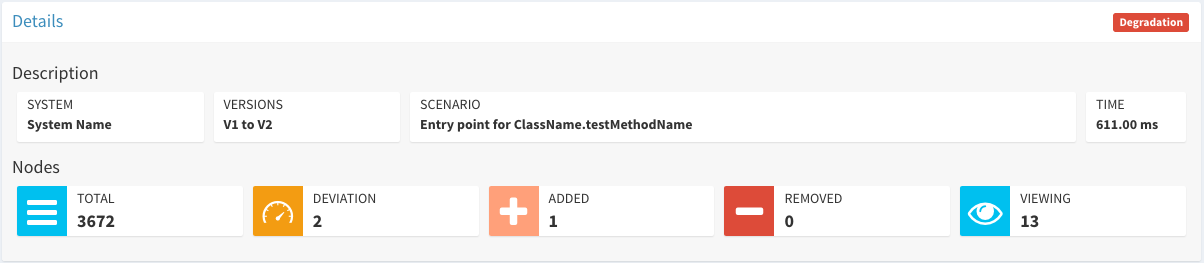
\includegraphics[scale=0.37]{Imagens/detalhes_grafo_chamadas.png}}
   \textsf{\caption[Seção de detalhes do grafo de chamadas.]{Seção de detalhes do grafo de chamadas.\label{fig:detalhes-grafo-chamadas}}}
\end{figure}

Na figura \ref{fig:detalhes-grafo-chamadas}, é mostrada uma visão geral sobre o cenário atual na visualização, contendo informações inerentes ao cenário. Para a seção \textit{Description}, as informações exibidas são:
\begin{itemize}
   \item \textit{System}: nome do sistema analisado;
   \item \textit{Versions}: versões do sistema que foram analisadas. É mostrado no formato \textit{<versionA>} to \textit{<versionB>}. Espera-se que a versão B, neste caso, seja posterior a versão A. No exemplo da figura, a versão V2 (\textit{versionB}) é posterior a versão V1 (\textit{versionA});
   \item \textit{Scenario}: exibe o nome do cenário analisado;
   \item \textit{Time}: mostra o tempo de execução do cenário na versão mais recente. A diferença de tempo entre as duas versões vai guiar o que será exibido na barra de títulos da figura. No exemplo mostrado, o tempo na última versão degradou com relação ao tempo na versão anterior, sendo exibido, no canto superior direito, um rótulo em vermelho marcando o cenário como degradado (\textit{degradation}). Caso o tempo do cenário seja otimizado, é exibido um rótulo verde marcando-o como otimizado (\textit{optimization}).
\end{itemize}

Para a seção \textit{Nodes}, as informações são as seguintes:
\begin{itemize}
   \item \textit{Total}: mostra o número total de nós do cenário. Vale salientar que cada nó representa um método executado durante a hierarquia de chamadas do cenário. Pode acontecer de nós diferentes representarem o mesmo método. Isso pode acontecer porque o mesmo método pode ser chamado hierarquias de chamadas diferentes;
   \item \textit{Deviation}: exibe o número de nós que tiveram algum desvio de desempenho. Para que um determinado nó seja considerado com desvio de desempenho, ele (i) tem que estar presente nas duas versões analisadas e (ii) tenha ocorrido diferenças, para mais ou para menos, no seu desempenho durante a execução do cenário nas versões analisadas;
   \item \textit{Added}: apresenta o número de nós que foram adicionados da versão anterior para a posterior. Ou seja, são os nós que não existiam na execução do cenário para a versão anterior e passaram a existir na execução da versão posterior;
   \item \textit{Removed}: o contrário do conceito anterior. São apresentados os nós que foram removidos da versão anterior para a posterior. Os nós removidos não são exibidos na visualização do grafo de chamadas;
   \item Viewing: apresenta a quantidade de nós que estão sendo mostrados no grafo de chamadas.
\end{itemize}

A segunda parte da visualização é o grafo de chamadas propriamente dito. Esse grafo, como mencionado, é composto de nós e arestas direcionadas que expõem os caminhos das chamadas dos métodos para o cenário analisado. Os nós, representados por caixas, possuem algumas características visuais, apresentadas adiante.

\begin{figure}[htb]
   \centering
   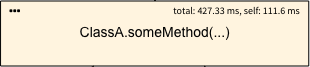
\includegraphics[scale=0.70]{Imagens/no_sem_desvio.png}
   \textsf{\caption[Nó que representa um método sem desvio de desempenho.]{Nó que representa um método sem desvio de desempenho.\label{fig:no-sem-desvio}}}
\end{figure}

O primeiro e mais básico tipo de nó é o que representa um método que não teve desvios de desempenho para o cenário e versões analisadas, apresentado na figura \ref{fig:no-sem-desvio}. As características desse nó são:\tabularnewline
\begin{itemize}
   \item \textit{Cor}: esta é a principal característica que diferencia os nós uns dos outros. No caso deste nó, a cor é marrom claro;
   \item \textit{Nome do nó}: posicionado ao centro, são mostrados o nome da classe e o nome do método executado, no formato \textit{ClassName.methodName()}. Para otimizar e evitar a exibição de grande quantidade de texto, o nome do pacote e os parâmetros do método foram ocultados, sendo estes representados por três pontos (...). Essa definição serve para todos os tipos de nós dessa visualização;
   \item \textit{Tempos de execução}: localizados no canto superior direito do nó, são apresentados dois tempos de execução: à esquerda, o tempo total do nó, que representa a soma dos tempos de execução dos nós filhos com o tempo do próprio nó. No exemplo da figura, o tempo total foi de 427,33 milissegundos; e à direita, o tempo do próprio nó, desconsiderando o tempo dos nós filhos. Na figura, o tempo foi de 111,6 milissegundos;
   \item \textit{Detalhes}: no canto superior esquerdo é exibido um ícone onde, ao passar o cursor do mouse, o usuário pode obter mais informações sobre o nó. No caso de um nó sem desvio de desempenho, as informações exibidas nesta seção são o nome do pacote e os parâmetros do método, se houver. A figura \ref{fig:detalhes-no-sem-desvio} a seguir mostra essa seção.
\end{itemize}

\begin{figure}[htb]
   \centering
   \frame{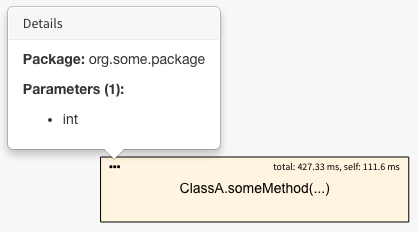
\includegraphics[scale=0.65]{Imagens/detalhes_no_sem_desvio.png}}
   \textsf{\caption[Seção de detalhes do nó sem desvio de desempenho.]{Seção de detalhes do nó sem desvio de desempenho.\label{fig:detalhes-no-sem-desvio}}}
\end{figure}

Quando um cenário possui nós que otimizaram o seu desempenho em relação à execução para a versão anterior, outros elementos visuais são acrescidos à visualização. A figura \ref{fig:no-otimizado} a seguir apresenta um nó otimizado:

\begin{figure}[htb]
   \centering
   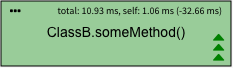
\includegraphics[scale=0.70]{Imagens/no_otimizado.png}
   \textsf{\caption[Nó que representa um método com otimização de desempenho.]{Nó que representa um método com otimização de desempenho.\label{fig:no-otimizado}}}
\end{figure}

As características visuais deste nó, além das comentadas anteriormente, são:
\begin{itemize}
   \item \textit{Cor}: os nós que otimizaram o atributo de qualidade desempenho são mostrados em um tom de verde;
   \item \textit{Tempos de execução}: além dos tempos total e do próprio nó, um nó com desvio de desempenho, seja otimização ou degradação, apresenta a diferença entre os tempos de execução da versão anterior para a posterior entre parênteses, no canto superior direito. No exemplo da figura, o nó melhorou o seu tempo em 32,66 milissegundos;
   \item \textit{Setas}: no canto inferior direito são mostradas setas indicativas de quão forte ou fraca foi a variação de desempenho. No caso de nós com otimização, são exibidas setas verdes apontadas para cima, onde cada uma delas representa 25\% de desvio do tempo com relação à versão anterior. Sendo assim, uma única seta representa um desvio de 0 a 25\%, duas setas de 25\% a 50\%, três setas de 50\% a 75\% e quatro setas de 75\% ou superior. No exemplo apresentado na figura \ref{fig:no-otimizado}, a otimização se deu entre 50\% e 75\% do desempenho anterior;
   \item \textit{Detalhes}: esta seção para os nós com otimização de desempenho possui informações diferentes das relatadas anteriormente, como podem ser vistas na figura \ref{fig:detalhes-no-otimizado}. Além das informações sobre o pacote e os parâmetros, também são apresentadas sobre os tempos de execução da versão anterior e posterior, além da variação de tempo.
\end{itemize}

\begin{figure}[htb]
   \centering
   \frame{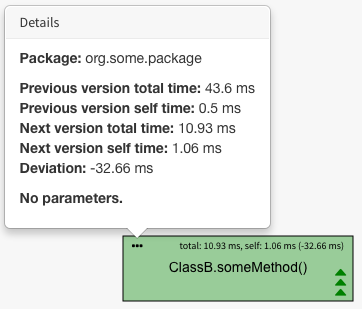
\includegraphics[scale=0.65]{Imagens/detalhes_no_otimizado.png}}
   \textsf{\caption[Seção de detalhes do nó com otimização de desempenho.]{Seção de detalhes do nó com otimização de desempenho.\label{fig:detalhes-no-otimizado}}}
\end{figure}

 A visualização também é capaz de apontar se determinado nó teve o seu desempenho degradado com relação à versão anterior. A figura \ref{fig:no-degradado} apresenta um nó degradado:

\begin{figure}[htb]
   \centering
   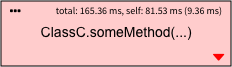
\includegraphics[scale=0.70]{Imagens/no_degradado.png}
   \textsf{\caption[Nó que representa um método com degradação de desempenho.]{Nó que representa um método com degradação de desempenho.\label{fig:no-degradado}}}
\end{figure}

As características visuais deste nó são bem semelhantes às apresentadas para os nós otimizados:
\begin{itemize}
   \item \textit{Cor}: os nós que degradaram o desempenho são mostrados em vermelho claro;
   \item \textit{Tempos de execução}: também são exibidos os tempos de execução total, do próprio nó e o desvio de desempenho. No exemplo, o nó degradou o tempo em 9,36 milissegundos;
   \item \textit: as setas indicativas de variação de desempenho para nós de degradação são apontadas para baixo, de cor vermelha. No exemplo, a degradação se deu entre 0 e 25\% do desempenho anterior;
   \item \textit{Detalhes}: esta seção possui as mesmas informações dos nós relatados até aqui, como podem ser vistas na figura \ref{fig:detalhes-no-degradado} a seguir.
\end{itemize}

\begin{figure}[htb]
   \centering
   \frame{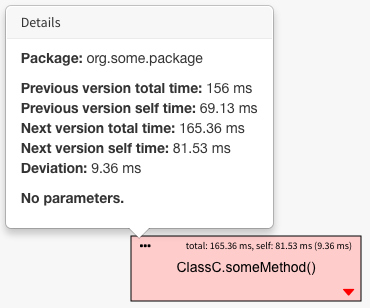
\includegraphics[scale=0.65]{Imagens/detalhes_no_degradado.png}}
   \textsf{\caption[Seção de detalhes do nó com degradação de desempenho.]{Seção de detalhes do nó com degradação de desempenho.\label{fig:detalhes-no-degradado}}}
\end{figure}

Um cenário pode apresentar, para diferentes versões, nós de chamadas de métodos que estão presentes na versão posterior, mas que não existiam na versão anterior. A visualização representa esses nós como mostra a figura \ref{fig:no-adicionado}. A descrição dos atributos visuais é a que segue:

\begin{figure}[htb]
   \centering
   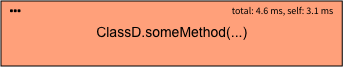
\includegraphics[scale=0.70]{Imagens/no_adicionado.png}
   \textsf{\caption[Nó que representa um método adicionado.]{Nó que representa um método adicionado.\label{fig:no-adicionado}}}
\end{figure}

\begin{itemize}
   \item \textit{Cor}: os nós que degradaram o desempenho são mostrados na cor salmão claro;
   \item \textit{Tempos de execução}: os tempos de execução total e do próprio nó são exibidos. No exemplo, o nó tem tempo total de em 4,6 milissegundos e o seu tempo é de 3,1 milissegundos.
   \item \textit{Detalhes}: nos nós adicionados, os detalhes possuem as mesmas informações exibidas para os nós de degradação ou de otimização. No entanto, uma mensagem é exibida em vermelho indicando que o nó adicionado é um potencial causador da degradação de desempenho do cenário. A figura \ref{fig:detalhes-no-adicionado} adiante apresenta esta seção.
\end{itemize}

\begin{figure}[htb]
   \centering
   \frame{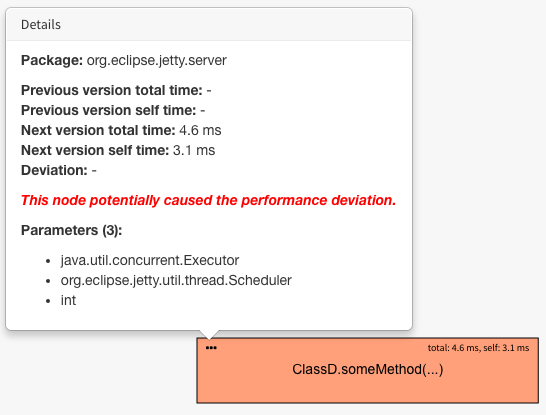
\includegraphics[scale=0.65]{Imagens/detalhes_no_adicionado.png}}
   \textsf{\caption[Seção de detalhes do nó adicionado.]{Seção de detalhes do nó adicionado.\label{fig:detalhes-no-adicionado}}}
\end{figure}

Além dos que representam métodos com ou sem desvio de desempenho, e métodos adicionados, há um tipo de nó que representa um agrupamento de vários outros: o agrupado. Assim, os que não estão diretamente relacionados com nós de desvio ou adicionados, são omitidos e representados por um único nó agrupado. A figura \ref{fig:no-agrupamento} a seguir ilustra esse tipo de nó, seguido da descrição dos seus atributos visuais.

\begin{figure}[htb]
   \centering
   \frame{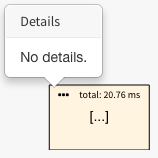
\includegraphics[scale=0.70]{Imagens/no_agrupamento.png}}
   \textsf{\caption[Nó que representa um agrupamento de outros nós.]{Nó que representa um agrupamento de outros nós.\label{fig:no-agrupamento}}}
\end{figure}

\begin{itemize}
   \item \textit{Cor}: os nós de agrupamento são mostrados na cor marrom claro;
   \item \textit{Nome do nó}: posicionado ao centro, é exibido o texto \textit{[...]};
   \item \textit{Tempos de execução}: é exibido o tempo de execução total que representa a soma de todos os tempos de execução dos nós contidos no agrupamento. No exemplo, o tempo total é de 20,76 milissegundos;
   \item \textit{Detalhes}: como pode ser percebido na imagem, este tipo de nó não possui detalhes a serem apresentados.
\end{itemize}

As propriedades visuais apresentadas para a visualização do grafo de chamadas incluem, em suma, duas partes: (i) seção de detalhes, contendo informações gerais sobre o cenário; e (ii) seção do grafo de chamadas, onde a execução dos métodos é representada através de nós e arestas. Esta seção é a mais importante desta visualização, contendo características visuais que diferem os nós de acordo com sua classificação. Um resumo dessas características é apresentado na tabela \ref{tab:resumo-caracteristicas-nos} a seguir.

\begin{table}[!htb]
   \textsf{\caption{Resumo das características visuais dos nós.\label{tab:resumo-caracteristicas-nos}}}
   \centering
   \medskip
   \begin{tabular}{c|c|c|c|c}
   \textbf{Tipo} & \textbf{Cor}   & \textbf{\begin{tabular}[c]{@{}c@{}}Tempos de\\ Execução\end{tabular}} & \textbf{Setas}                                                  & \textbf{Detalhes}                                                                     \\ \hline
   Sem desvio    & Marrom claro   & Total e próprio                                                       & Sem setas                                                       & \begin{tabular}[c]{@{}c@{}}Pacotes e \\ parâmetros\end{tabular}                       \\ \hline
   Degradado     & Vermelho claro & \begin{tabular}[c]{@{}c@{}}Total, próprio\\ e desvio\end{tabular}     & \begin{tabular}[c]{@{}c@{}}Vermelhas,\\ para baixo\end{tabular} & \begin{tabular}[c]{@{}c@{}}Pacotes, tempos\\ de execução e \\ parâmetros\end{tabular} \\ \hline
   Otimizado     & Verde claro    & \begin{tabular}[c]{@{}c@{}}Total, próprio\\ e desvio\end{tabular}     & \begin{tabular}[c]{@{}c@{}}Verdes,\\ para cima\end{tabular}     & \begin{tabular}[c]{@{}c@{}}Pacotes, tempos\\ de execução e \\ parâmetros\end{tabular} \\ \hline
   Adicionado    & Salmão claro   & Total e próprio                                                       & Sem setas                                                       & \begin{tabular}[c]{@{}c@{}}Pacotes, tempos\\ de execução e \\ parâmetros\end{tabular} \\ \hline
   Agrupado      & Marrom claro   & Total                                                                 & Sem setas                                                       & Sem detalhes
   \end{tabular}
\end{table}

\subsubsection{Interação} \label{subsec:interacao}

Esta visualização exibe um conjunto de informações que a torna capaz de indicar os métodos que potencialmente foram responsáveis por desvios de desempenho de um determinado cenário. Contudo, o usuário pode interagir com o grafo: (i) obtendo mais informações sobre um nó, passando o cursor do \textit{mouse} por cima do ícone de detalhes, como mostrado anteriormente; e (ii) executando o efeito de \textit{zoom} sobre o grafo para afastar ou aproximar a visualização. Esse efeito pode fazer com que o grafo seja comportado novamente na área de desenho.

\subsection{Funcionamento} \label{subsec:funcionamento-visualizacao-3}

A visualização utiliza os artefatos de saída gerados após a execução completa do \textit{PerfMiner}, de modo que se configura como mais uma etapa da ferramenta. A figura \ref{fig:perfminer-fase4} ilustra essa etapa. A extensão foi implementada em uma aplicação web, conforme explanado anteriormente e ilustrado na figura \ref{fig:funcionamento-geral-visualizacoes}. Embora o funcionamento mostrado nessa figura seja geral, são necessários processamentos específicos para esta visualização, a fim de tratar os dados para serem exibidos para o usuário.

Para esta visualização, seguindo o funcionamento mostrado na figura \ref{fig:funcionamento-geral-visualizacoes}, o usuário realiza a requisição para esta visualização, passando como parâmetros o nome do sistema e as duas versões (passo 1). Os passos 2 e 3, em detalhes, é exibido na figura \ref{fig:passos-2-3-grafo-chamadas}.

\begin{figure}[!htb]
   \centering
   \frame{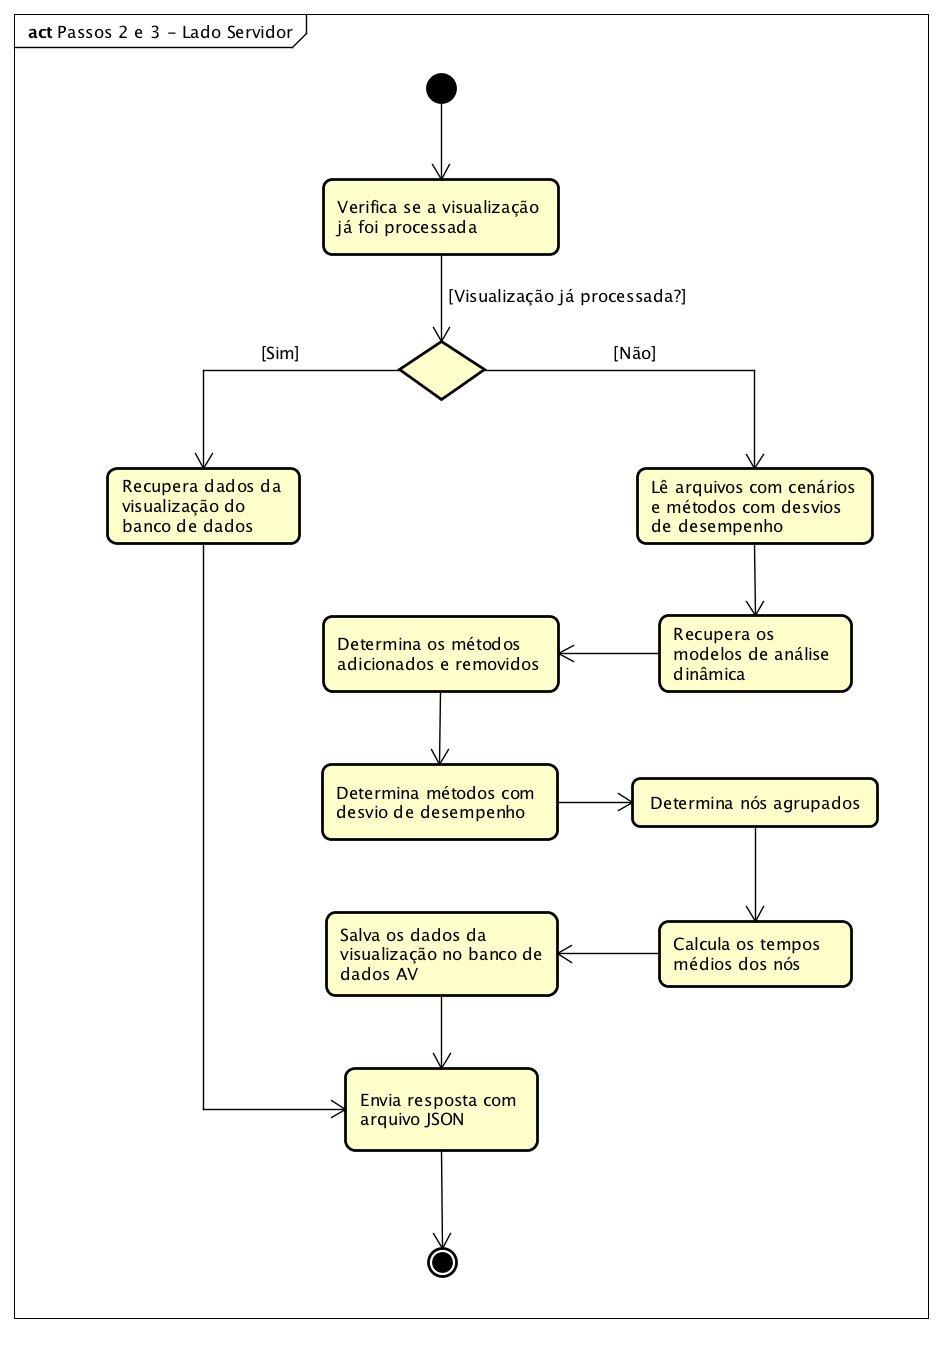
\includegraphics[scale=0.45]{Imagens/visualizacao_3_fase_2_e_3.png}}
   \textsf{\caption[Passos 2 e 3 da visualização grafo de chamadas.]{Passos 2 e 3 da visualização grafo de chamadas.\label{fig:passos-2-3-grafo-chamadas}}}
\end{figure}

O processo se inicia quando o servidor recebe a requisição do usuário, solicitando a visualização do grafo de chamadas para determinadas versões de um sistema. Ao receber, a aplicação verifica se a visualização requerida já foi processada anteriormente, consultando-a no banco de dados QAV. Em caso positivo, os dados são recuperados, o arquivo JSON é montado e enviado na resposta do servidor, e o processo acaba.

Caso a visualização ainda não tenha sido processada, os arquivos de saída do \textit{PerfMiner} contendo informações sobre os cenários e métodos com desvio de desempenho são lidos e os modelos de análise dinâmica de ambas as versões são recuperados do banco de dados DAM. Esse modelo é formado por um grafo com todos os nós de chamadas dinâmico que representa cada execução do cenário.

De posse dos nós recuperados, são determinados os métodos que foram adicionados ou removidos comparando os nós da versão atual com os da anterior. Depois disso, a partir dos métodos indicados pelos arquivos de saída do \textit{PerfMiner}, são determinados os nós com desvios de desempenho, seja degradação ou otimização.

Na extensão, os nós identificados como adicionados e com desvio são candidatos a serem exibidos. Optou-se por apresentar apenas os nós com desvio, nós adicionados e alguns nós sem desvio de desempenho, mas que garantem o entendimento do grafo, de modo que poucos nós são renderizados no navegador do usuário. Essa decisão levou em consideração a quantidade de nós de um cenário, que facilmente pode passar dos milhares, o desempenho da própria aplicação web e a eficácia no entendimento da visualização por parte do usuário. Espera-se que, com menos nós exibidos, os usuários consigam entender e acompanhar mais claramente a evolução do atributo de qualidade de desempenho.

Após determinar os nós com desvios de desempenho, são criados nós de agrupamento para representar os nós que não serão exibidos na visualização. Depois disso, os tempos médios dos nós a serem exibidos são calculados, levando em consideração todas as ocorrências do método no cenário. Após, os dados do processamento são salvos no banco de dados QAV e, por fim, o arquivo JSON que dá suporte à visualização é montado e enviado como resposta do servidor, e o processo acaba.

Quando o usuário recebe a resposta, há um procedimento executado no seu navegador, que recebe e processa o arquivo JSON e, ao final, renderiza o grafo de chamadas. Esse processo representa o passo 5 da figura \ref{fig:funcionamento-geral-visualizacoes} está exposto em detalhes na figura \ref{fig:passo-5-grafo-chamadas} adiante. O início ocorre ao receber o arquivo do servidor e a primeira atividade é criar a área de desenho que abrigará o grafo. Nessa atividade são considerados a altura e largura do monitor do usuário, de modo que a área útil de apresentação seja compatível com a área do monitor.

\begin{figure}[!htb]
   \centering
   \frame{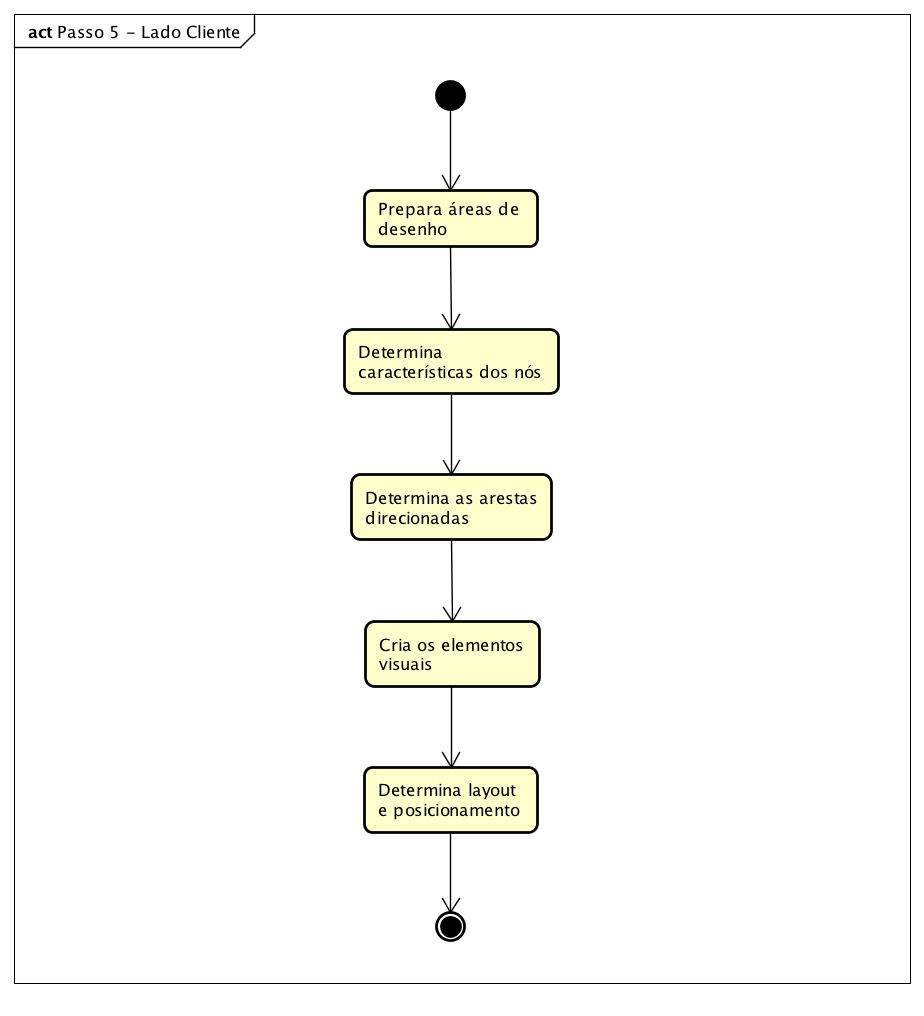
\includegraphics[scale=0.50]{Imagens/visualizacao_3_fase_5.png}}
   \textsf{\caption[Passos 5 da visualização grafo de chamadas.]{Passos 5 da visualização grafo de chamadas.\label{fig:passo-5-grafo-chamadas}}}
\end{figure}

Após isso, as características dos nós contidos no arquivo JSON são determinadas. Para cada um deles, são determinados: (i) a altura e largura da sua caixa, que é diretamente proporcional ao tamanho do nome a ser exibido. Vale salientar que o pacote da classe é omitido para a exibição do nome; (ii) a cor, que depende do seu tipo; (iii) os tempos de execução total e, caso pertinente, o do próprio nó e o de desvio; (iv) as setas, que dependem do seu tipo e da porcentagem de desvio do tempo de execução ocorrida de uma versão para outra; e (v) os detalhes, que dependem do tipo do nó.

Depois, as arestas são determinadas de acordo com a relação de nós pais e filhos contidos no arquivo. Elas são direcionadas do nó pai para os filhos, indicando a hierarquia de chamadas.

Com a definição dos nós e suas características, e das arestas, a próxima atividade do processo é criar os elementos visuais na área de desenho, para, posteriormente, determinar o \textit{layout} (conforme citado anteriormente, o \textit{layout} utilizado é em árvore) e posicionamento dos nós. Por fim, o grafo de chamadas é renderizado para o usuário.

\subsection{Exemplo de Uso da Ferramenta: Jetty} \label{subsec:exemplo-uso-jetty}

Foi realizado um estudo de caso para exemplificar o uso das visualizações. Para tanto, foi utilizado duas versões da aplicação Jetty \cite{Jetty2016}: 9.2.6 e 9.3.0.M1. Esse sistema faz parte do Projeto Eclipse e é um \textit{framework open-source} que provê um servidor web além de um servlet container Java. Essa aplicação foi escolhida para o estudo de caso pois todos os tipos de nós foram capazes de ser exemplificados.

Para a primeira fase do \textit{PerfMiner}, a análise dinâmica, todos os testes automatizados foram considerados cenários. Como os testes são implementados em JUnit 4, o aspecto interceptou todos os métodos marcados com a anotação \texttt{@Test} como métodos de entrada de um cenário. A análise dinâmica, como mencionado anteriormente, foi executada no mesmo computador para ambas as versões, nas mesmas condições e com todos os serviços não essenciais desabilitados. A suíte de testes do Jetty foi executada 30 vezes para que as medições de desempenho fossem mais precisas em termos de tempo de execução \cite{Pinto2015}.

A resultado da análise foi um total de 11 cenários, sendo 7 com degradação do desempenho e 4 com otimização. No grafo gerado, é possível que dois nós representem o mesmo método, indicando duas execuções, e as arestas direcionadas representam invocações entre os métodos. A figura \ref{fig:exemplo-degradacao} exemplifica o grafo de um cenário com degradação.

\begin{figure}[!htb]
   \centering
   \frame{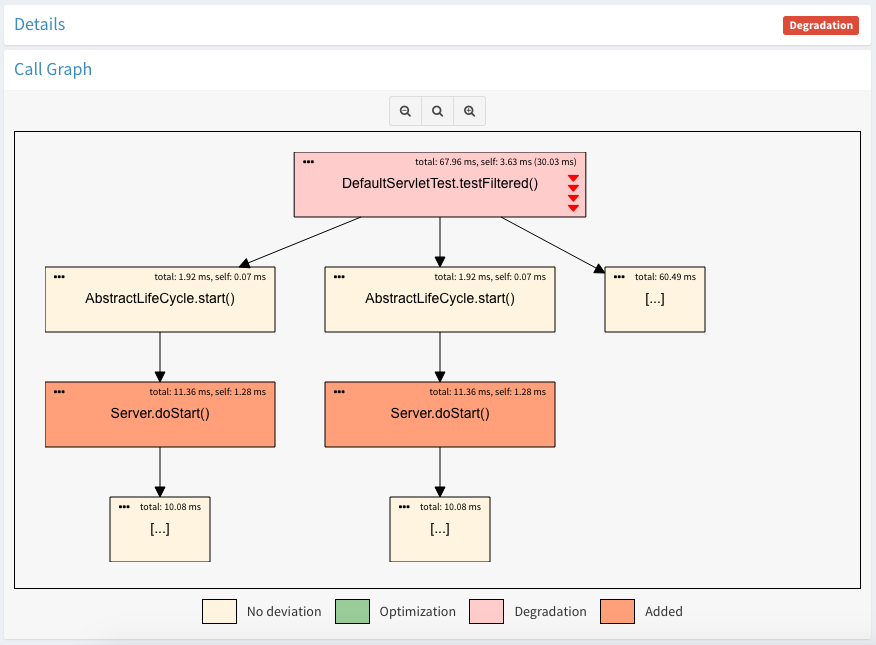
\includegraphics[scale=0.52]{Imagens/exemplo_degradacao.png}}
   \textsf{\caption[Grafo de chamadas de um cenário com degradação de desempenho.]{Grafo de chamadas de um cenário com degradação de desempenho.\label{fig:exemplo-degradacao}}}
\end{figure}

O grafo exibido destaca que o nó raiz, \texttt{DefaultServletTest.testFiltered()}, teve uma degradação de desempenho de mais de 75\%, indicado pela cor do nó, vermelho claro, e pelas quatro setas vermelhas para baixo. É possível notar também que dois nós que representam o método \texttt{Server.doStart()} foram adicionados. Isso significa que durante a execução do cenário \texttt{Entry point for DefaultServletTest.testFiltered} duas chamadas a esse método foram efetuadas na versão 9.3.0.M1, e elas não existiam na versão 9.3.6. Os nós adicionados são indicados como potenciais causadores de degradação de desempenho, de modo que, possivelmente, esses nós influenciaram na degradação do raiz. Na visualização há nós que não têm relação com os desvios, representados como agrupados, e nós sem desvio, representados na cor marrom claro.

Na mesma figura, além do próprio grafo, na parte superior da seção \textit{Call Graph} é encontrada uma barra de ferramentas com botões de \textit{Zoom Out}, \textit{Zoom to Fit} e \textit{Zoom In}; e na parte inferior é exibida uma legenda ajudando os usuários a identificarem os nós do grafo. Os botões de \textit{zoom} e a legenda são exibidos para todos os grafos, independente da quantidade de nós ou do tipo de desvio ocorrido.

Na figura \ref{fig:exemplo-detalhes-degradacao} adiante, a seção \textit{Details} desse cenário é exibida expandida, indicando, no rótulo, que o cenário teve o seu desempenho degradado entre as versões, e que o total de nós para esse cenário foi de 1695.

\begin{figure}[!htb]
   \centering
   \frame{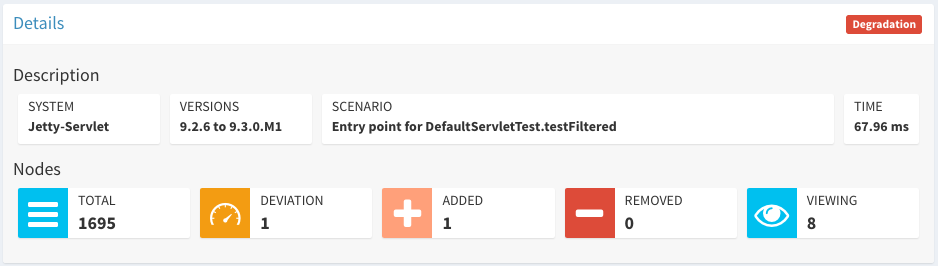
\includegraphics[scale=0.48]{Imagens/exemplo_detalhes_degradacao.png}}
   \textsf{\caption[Detalhes de um cenário com degradação de desempenho.]{Detalhes de um cenário com degradação de desempenho.\label{fig:exemplo-detalhes-degradacao}}}
\end{figure}

A figura \ref{fig:exemplo-otimizacao} a seguir apresenta o cenário \texttt{Entry point for ServletContextHandler\\Test.testFallThrough} com otimização de desempenho. Dois nós contribuíram para esse desvio, identificados pela cor verde claro: \texttt{Server.doStart()} e \texttt{ServletContextHandler.\\relinkHandlers()}. No primeiro, a variação foi entre 50\% e 75\%, ao passo que no segundo foi de mais de 75\%. Há ainda a representação de nós agrupados e sem desvio.

\begin{figure}[!htb]
   \centering
   \frame{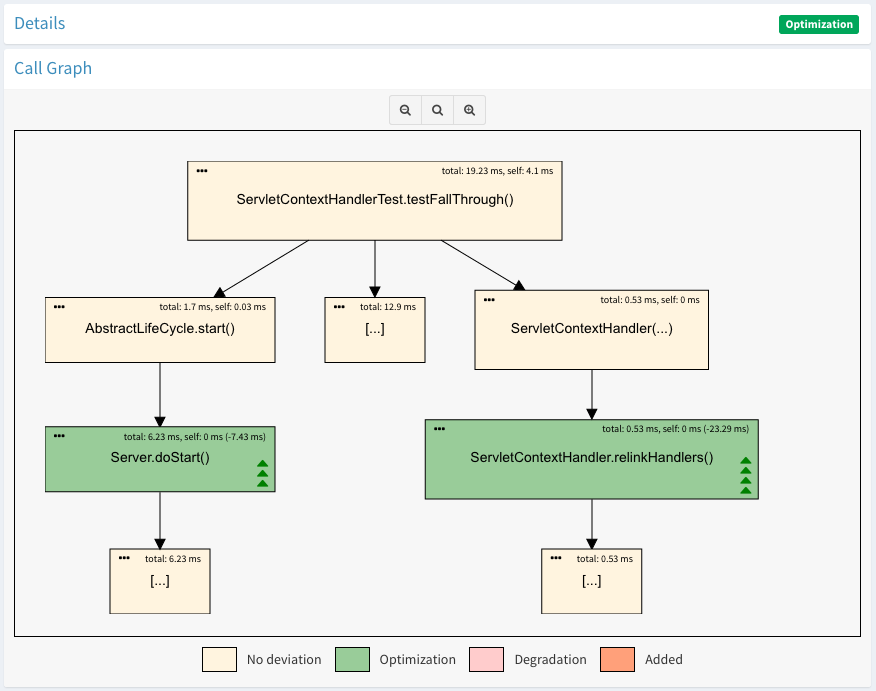
\includegraphics[scale=0.52]{Imagens/exemplo_otimizacao.png}}
   \textsf{\caption[Grafo de chamadas de um cenário com otimização de desempenho.]{Grafo de chamadas de um cenário com otimização de desempenho.\label{fig:exemplo-otimizacao}}}
\end{figure}

\begin{figure}[!htb]
   \centering
   \frame{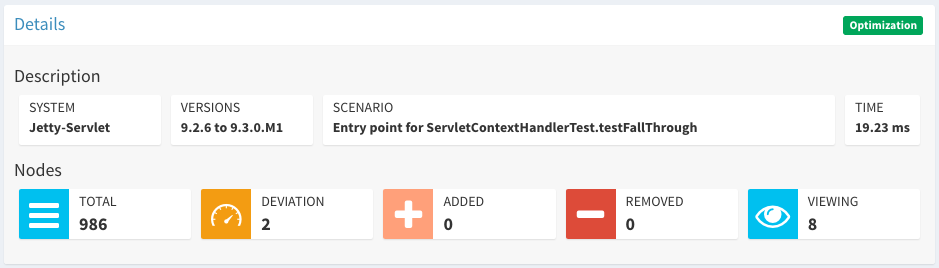
\includegraphics[scale=0.48]{Imagens/exemplo_detalhes_otimizacao.png}}
   \textsf{\caption[Detalhes de um cenário com otimização de desempenho.]{Detalhes de um cenário com otimização de desempenho.\label{fig:exemplo-detalhes-otimizacao}}}
\end{figure}

A seção \textit{Details} expandida pode ser vista na figura \ref{fig:exemplo-detalhes-otimizacao}. O rótulo de otimização é exibido no canto superior esquerdo indicando o tipo de desvio ocorrido no cenário. A figura indica um total de 986 nós para esse cenário.

A tabela \ref{tab:jetty-v9.2.6-v9.3.0.M1} a seguir mostra uma lista com todos os cenários para o sistema Jetty, versões 9.2.6 para 9.3.0.M1. Nela, são exibidas as porcentagens de desvio de degradação ou otimização para os cenários.

\begin{sidewaystable}[!htb]
   \textsf{\caption{Cenários para o Jetty, versões 9.2.6 para 9.3.0.M1.\label{tab:jetty-v9.2.6-v9.3.0.M1}}}
   \centering
   \medskip
   \begin{tabular}{l|c|c|c|c}
   \multicolumn{1}{c|}{\textbf{Nome}}                                                                                                       & \textbf{\begin{tabular}[c]{@{}c@{}}Tempo \\ v9.2.6 (ms)\end{tabular}} & \textbf{\begin{tabular}[c]{@{}c@{}}Tempo \\ v9.3.0.M1 (ms)\end{tabular}} & \textbf{\begin{tabular}[c]{@{}c@{}}Variação \\ (\%)\end{tabular}} & \textbf{\begin{tabular}[c]{@{}c@{}}Tipo de \\ Desvio\end{tabular}} \\ \hline
   \begin{tabular}[c]{@{}l@{}}Entry point for \\ DispatcherForwardTest.testQueryRetainedByForward\\ WithoutQuery\end{tabular}              & 569,26                                                                & 597,33                                                                   & 4,93                                                              & Degradação                                                         \\ \hline
   \begin{tabular}[c]{@{}l@{}}Entry point for \\ SSLAsyncIOServletTest.testAsyncIOWritesWith\\ Aggregation\end{tabular}                    & 549,21                                                                & 587,55                                                                   & 6,98                                                              & Degradação                                                         \\ \hline
   \begin{tabular}[c]{@{}l@{}}Entry point for \\ AsyncServletLongPollTest.testSuspendedRequest\\ CompletedByAnotherRequest\end{tabular}    & 620,36                                                                & 634,60                                                                   & 2,29                                                              & Degradação                                                         \\ \hline
   Entry point for DefaultServletTest.testFiltered                                                                                         & 37,93                                                                 & 67,96                                                                    & 79,17                                                             & Degradação                                                         \\ \hline
   \begin{tabular}[c]{@{}l@{}}Entry point for \\ ServletContextHandlerTest.testReplaceServlet\\ HandlerWithoutServlet\end{tabular}         & 429,60                                                                & 453,96                                                                   & 5,67                                                              & Degradação                                                         \\ \hline
   \begin{tabular}[c]{@{}l@{}}Entry point for \\ AsyncContextListenersTest.testAsyncDispatch\\ AsyncCompletePreservesListener\end{tabular} & 601,83                                                                & 622,96                                                                   & 3,51                                                              & Degradação                                                         \\ \hline
   \begin{tabular}[c]{@{}l@{}}Entry point for \\ AsyncIOServletTest.testAsyncWriteThrowsError\end{tabular}                                 & 599,10                                                                & 611,00                                                                   & 1,98                                                              & Degradação                                                         \\ \hline
   \begin{tabular}[c]{@{}l@{}}Entry point for \\ DispatcherForwardTest.testQueryAggregatesWith\\ FormByForwardWithoutQuery\end{tabular}    & 26,46                                                                 & 20,76                                                                    & 21,54                                                             & Otimização                                                         \\ \hline
   \begin{tabular}[c]{@{}l@{}}Entry point for \\ ServletContextHandlerTest.testFallThrough\end{tabular}                                    & 52,00                                                                 & 19,23                                                                    & 63,01                                                             & Otimização                                                         \\ \hline
   \begin{tabular}[c]{@{}l@{}}Entry point for \\ AsyncContextListenersTest.testListenerCleared\\ OnSecondRequest\end{tabular}              & 23,90                                                                 & 17,16                                                                    & 28,20                                                             & Otimização                                                         \\ \hline
   \begin{tabular}[c]{@{}l@{}}Entry point for \\ ServletContextHandlerTest.testAddServletAfterStart\end{tabular}                           & 55,56                                                                 & 20,40                                                                    & 63,28                                                             & Otimização                                                     
   \end{tabular}
\end{sidewaystable}

A maior variação absoluta foi para o cenário \texttt{Entry point for DefaultServletTest\\.testFiltered}, uma degradação de 79,17\%. Como destacado na figura \ref{fig:exemplo-degradacao}, dois nós com tempos significantes com relação ao cenário foram adicionados, provavelmente, causando a degradação. O gráfico \ref{fig:grafico-jetty-v9.2.6-v9.3.0.M1} adiante exibe a porcentagem de variação de desempenho.

\begin{sidewaysfigure}[!htb]
   \centering
   \frame{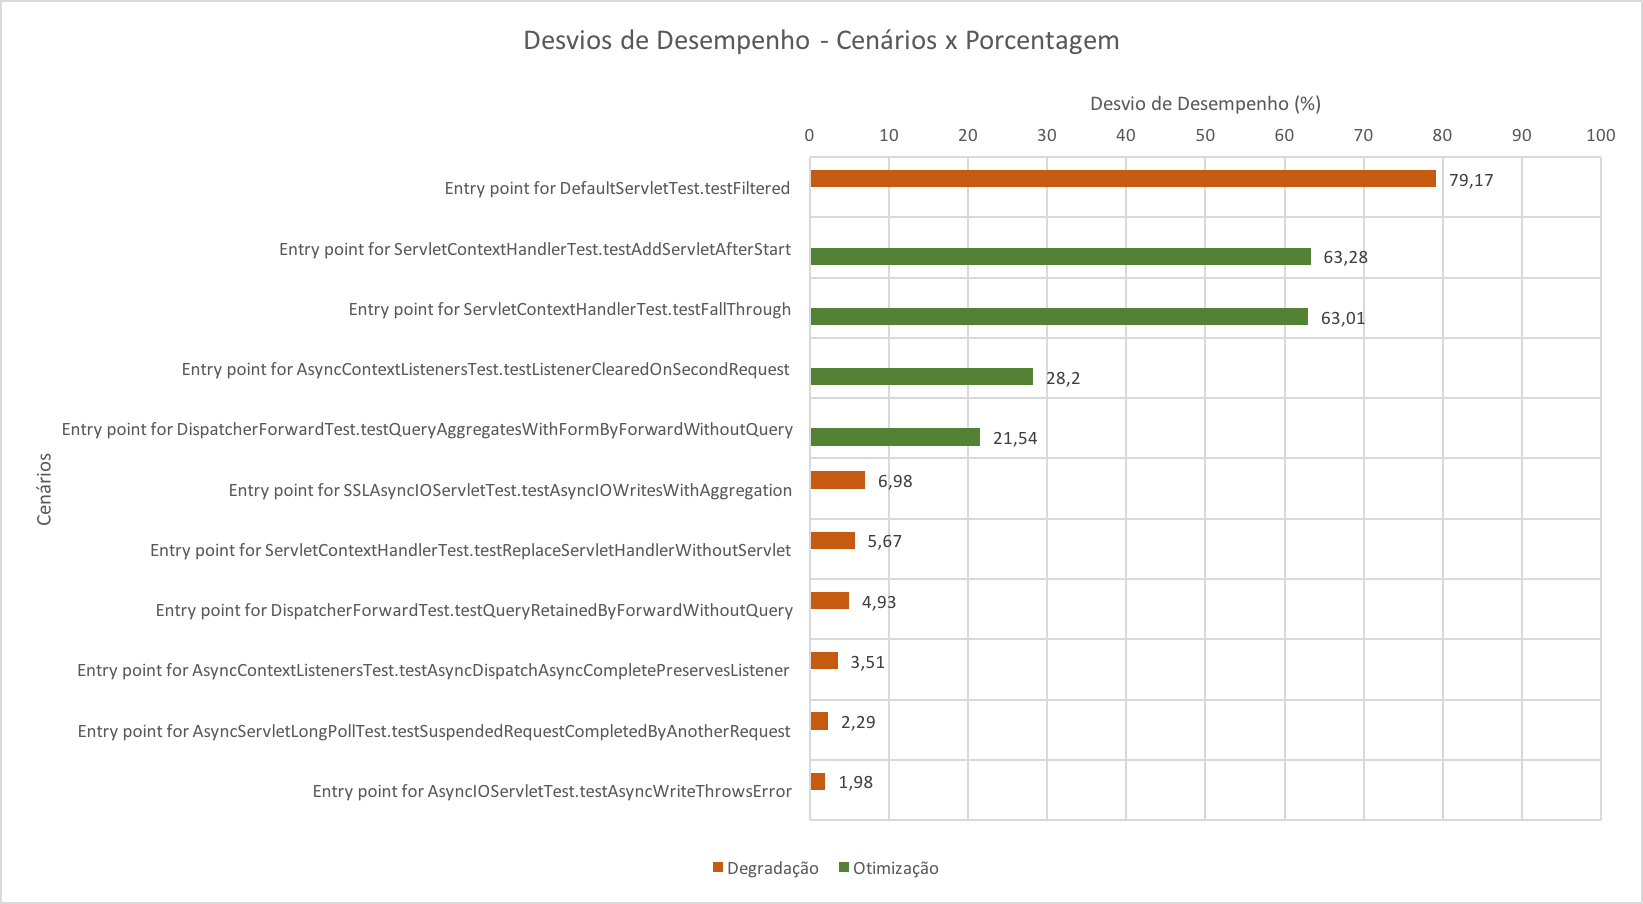
\includegraphics[scale=0.80]{Imagens/grafico_jetty_v926_v931M1.png}}
   \textsf{\caption[Porcentagem de desvios de desempenho para o Jetty, versões 9.2.6 para 9.3.0.M1.]{Porcentagem de desvios de desempenho para o Jetty, versões 9.2.6 para 9.3.0.M1.\label{fig:grafico-jetty-v9.2.6-v9.3.0.M1}}}
\end{sidewaysfigure}

\section{Considerações} \label{sec:consideracoes-cap3}


Um dos principais desafios do processo de manutenção de um software é compreendê-lo adequadamente, em especial, a sua arquitetura. A falta de acompanhamento da evolução da arquitetura ao longo do tempo pode levar a sua degradação, impactando os seus atributos de qualidade. Este capítulo apresentou visualizações de arquitetura de software que visam tornar direta e fácil a monitoração da evolução arquitetural, com relação ao atributo de qualidade de desempenho. Uma vez que as ferramentas existentes se mostram complexas ou ineficientes para essa finalidade, as visualizações foram propostas a serem implementadas como extensões da ferramenta \textit{PerfMiner}. Em suma, são as seguintes:
\begin{enumerate}[(i)]
   \item \textit{Evolução do Desempenho}: a evolução do atributo de qualidade de desempenho pode ser acompanhada em outra visualização, que mostra, para cada versão do sistema, se este degradou, otimizou ou manteve estável o seu desempenho;
   \item \textit{Sumarização dos Cenários}: a sumarização dos cenários com desvio de desempenho objetiva mostrar, de maneira sucinta, quais cenários analisados tiveram desvio de desempenho, seja degradação ou otimização;
   \item \textit{Grafo de Chamadas}: a visualização do grafo de chamadas exibe, para cada cenário, as chamadas dos métodos que tiveram desvio de desempenho. Dessa forma, o usuário pode localizar em qual trecho de código da execução do cenário houve o desvio.
\end{enumerate}

Foi mostrado os detalhes da visualização do grafo de chamadas, que visa exibir, para dadas duas versões de um sistema, os métodos que potencialmente causaram o desvio de desempenho para um determinado cenário. Nesta visualização, os métodos são apresentados em um grafo direcionado de chamadas com propriedades visuais que destacam quais dos métodos mostrados tiveram desvios de desempenho.

É importante frisar que a implementação das visualizações ainda não está finalizada. As duas primeiras mencionadas neste capítulo, evolução do desempenho e sumarização dos cenários, ainda estão em fase de concepção, ao passo que a terceira, grafo de chamadas, está em fase de conclusão. Para esta última, ainda serão adicionados, na seção de detalhes dos nós, \textit{links} para os \textit{commits} e tarefas que alteraram o método representado. Para cada método com desvio, serão recuperados os \textit{commits} do sistema de controle de versões e verificado quais commits alteraram linhas dentro do método detectado. Para cada um dos que alteraram, o número da respectiva tarefa é procurado na mensagem de \textit{commit}. Este número é usado para procurar a tarefa no sistema de gerenciamento de tarefas em busca de informações extras, como o seu tipo.

\section{Ameaças à validade} \label{sec:ameacas}